% !TEX program = lualatex
\documentclass[paper=a4,fontsize=9pt]{jlreq}

\usepackage[top=13mm,bottom=13mm,left=14mm,right=14mm]{geometry}
\usepackage{graphicx}
\usepackage{booktabs}
\usepackage{amsmath}
\usepackage{caption}
\usepackage{subcaption}
\usepackage{enumitem}
\usepackage{xcolor}

\captionsetup{font=small,labelfont=bf}
\setlist[itemize]{leftmargin=1.2em,itemsep=0.1em,topsep=0.1em}
\setlength{\parindent}{1em}
\setlength{\parskip}{0.15em}
\renewcommand{\arraystretch}{1.05}

\title{\vspace{-1.4em}低信頼エッジキャッシュ環境における\\近隣協調型フォールバック制御の初期検討}
\author{進捗メモ}
\date{\today}

\begin{document}
\maketitle
\vspace{-2.5em}

\section{目的と検討対象}
本メモでは，低信頼エッジキャッシュ環境において，ローカル ES 集合のみではファイル復元に必要なチャンク数を満たせない場合のフォールバック方式を比較した初期結果を報告する．現在の段階では，正式な離散事象シミュレーションではなく，フォールバック制御ロジックの傾向を確認するための preliminary Monte Carlo simulation として位置づけている．評価対象は以下の三方式である．

\begin{itemize}
  \item \textbf{B0}: ローカル ES で復元できない場合，直接オリジンから不足チャンクを取得する方式．
  \item \textbf{B1}: ローカル ES で復元できない場合，常に近隣 ES 協調グループを探索し，失敗時にオリジンへフォールバックする方式．
  \item \textbf{B2}: 期待遅延に基づく近隣探索判定方式．近隣探索が有利と判断される場合のみ近隣 ES を探索する．
\end{itemize}

B2 では，近隣復元成功確率を $P_s=\Pr(X\ge K),\ X\sim\mathrm{Binomial}(N_{\mathrm{nbr}},p_{\mathrm{nbr}})$ と近似し，近隣探索の期待遅延を次式で判定する．
\[
E_{\mathrm{nbr}}
=P_sT_{\mathrm{nbr}}+(1-P_s)(T_{\mathrm{probe}}+T_{\mathrm{origin}})
\le T_{\mathrm{origin}} .
\]
この条件を満たす場合に近隣探索を行い，満たさない場合は直接オリジン取得を選択する．

\section{シミュレーション設定}
共通設定として，要求は Zipf 分布（$\alpha=1.1$）に従うものとし，各条件で 10 trials，1 trial あたり 10,000 requests を用いた．復元に必要なチャンク数は $K=3$，ローカル ES 数は 3，近隣 ES グループサイズは 5 とした．評価指標は平均応答時間，95 パーセンタイル応答時間，オリジン非依存完了率，近隣探索失敗率である．

\begin{table}[h]
\centering
\caption{代表シナリオの設定．オリジン遅延増加シナリオは，現段階では queueing や service capacity を含む輻輳モデルではなく，オリジン取得遅延を増加させた stress setting である．}
\small
\begin{tabular}{lccc}
\toprule
シナリオ & ローカル ES 可用率 & 近隣 ES 可用率 & オリジン遅延 (ms) \\
\midrule
定常シナリオ & 0.82 & 0.82 & 180 \\
低信頼近隣 ES シナリオ & 0.82 & 0.25 & 180 \\
オリジン遅延増加シナリオ & 0.82 & 0.82 & 320 \\
\bottomrule
\end{tabular}
\end{table}

低信頼近隣 ES シナリオの近隣 ES 可用率 0.25 は，実測値ではなく，近隣探索が有効でない条件を観察するための stress setting である．また，ヒートマップでは，三つの代表シナリオで用いた近隣 ES 可用率およびオリジン遅延を含む範囲で感度分析を行った．

\newpage

\section{初期結果}
\begin{figure}[t]
\centering
\begin{subfigure}[t]{0.49\linewidth}
  \centering
  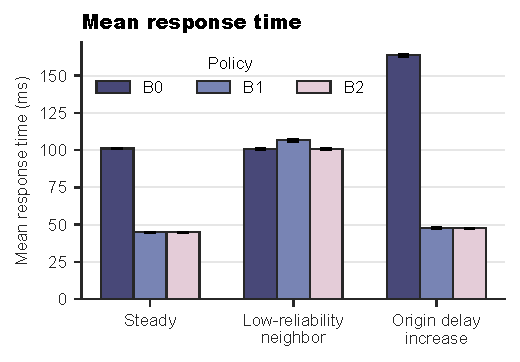
\includegraphics[width=\linewidth]{../results/figures/fig_phase1_memo_scenario_mean_response_time.pdf}
  \caption{Mean response time.}
\end{subfigure}
\hfill
\begin{subfigure}[t]{0.49\linewidth}
  \centering
  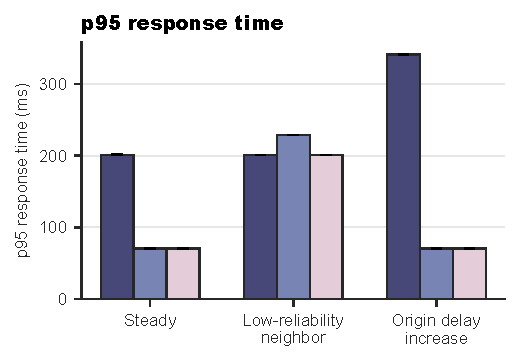
\includegraphics[width=\linewidth]{../results/figures/fig_phase1_memo_scenario_p95_response_time.pdf}
  \caption{95th percentile response time.}
\end{subfigure}
\caption{三つの代表シナリオにおける B0/B1/B2 の応答時間比較．エラーバーは repeated trials に基づく 95\% confidence interval を示す．}
\end{figure}

定常シナリオでは，近隣 ES が十分利用可能であるため，B1 と B2 はほぼ同等の性能を示した．これは，B2 の判定が多くの場合 B1 と同様に近隣探索を選択するためであり，想定通りの結果である．一方，低信頼近隣 ES シナリオでは，近隣復元成功確率が低く，近隣探索の期待遅延がオリジン取得遅延を上回るため，B2 は近隣探索を抑制する．このため，B1 で生じる「近隣探索後に失敗し，その後オリジンへ戻る」二重の遅延負担を避ける傾向が見られた．オリジン遅延増加シナリオでは，近隣 ES が利用可能な条件では B1/B2 が B0 より低い応答時間を示したが，B1 と B2 の差は小さい．

\begin{figure}[h]
\centering
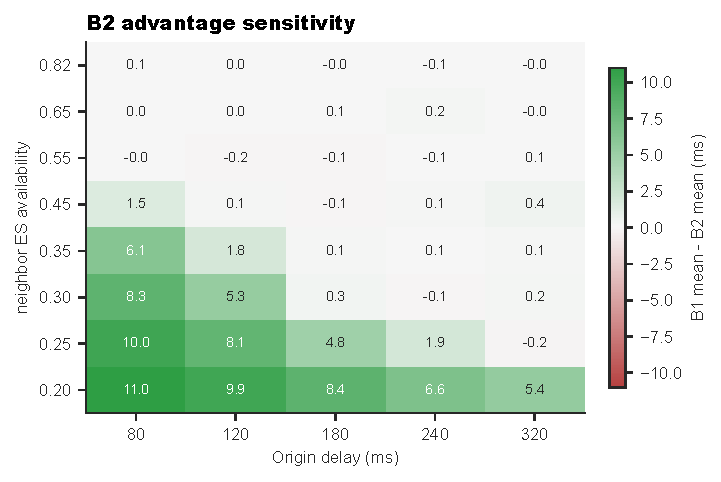
\includegraphics[width=0.68\linewidth]{../results/figures/fig_phase1_memo_b2_advantage_heatmap.pdf}
\caption{補足的な感度分析として，近隣 ES 可用率とオリジン遅延を変化させた場合の B2 advantage を示す．B2 advantage は B1 mean response time $-$ B2 mean response time と定義し，正の値は B2 が B1 より低遅延であることを示す．}
\end{figure}

\noindent\textbf{低信頼近隣 ES における挙動:}
\begin{center}
\small
\begin{tabular}{ll}
\toprule
Policy & 挙動 \\
\midrule
B1 & 近隣探索を行うため，失敗率が高くなる． \\
B2 & 期待遅延判定により，近隣探索を抑制する． \\
\bottomrule
\end{tabular}
\end{center}

\section{制限と次の段階}
現在のモデルでは，B2 の $P_s$ は簡略化された確率モデルであり，request arrival，service capacity，queueing delay は含んでいない．また，オリジン遅延増加シナリオはオリジン取得遅延を増加させたものであり，実際の server congestion を明示的にモデル化したものではない．さらに，コンテンツごとのキャッシュ配置，キャッシュ容量，キャッシュ置換もまだ導入していない．

次の段階では，コンテンツごとのキャッシュ配置やキャッシュ容量を導入する方向と，request arrival・service capacity・queueing delay を含む離散事象シミュレーションへ拡張する方向のどちらを優先すべきか，ご助言いただけますと幸いです．

\end{document}
